\PassOptionsToPackage{xetex}{xcolor}
\PassOptionsToPackage{xetex}{graphicx}
\documentclass[a4paper,landscape,headrule,footrule,xetex]{foils}


%%
%%% macros for 2009 Semester 1 HG 803
%%%
\newcommand{\logo}{~}
\newcommand{\header}[3]{%
  \title{\vspace*{-2ex} \large HG3051  Corpus Linquistics
    \\[2ex] \Large  \emp{#2} \\ \emp{#3}}
  \author{\blu{Francis Bond}   \\ 
    \normalsize  \textbf{Division of Linguistics and Multilingual Studies}\\
    \normalsize  \url{http://www3.ntu.edu.sg/home/fcbond/}\\
    \normalsize  \texttt{bond@ieee.org}}
  \MyLogo{HG3051 (2018)}
  \renewcommand{\logo}{#2}
  \hypersetup{
    pdfinfo={
      Author={Francis Bond},
      Title={#1: #2},
      Subject={HG3051: Corpus Linguistics},
      Keywords={Corpus Linguistics},
      License={CC BY 4.0}
    }
  }
  \date{#1 \\ \url{https://github.com/bond-lab/Corpus-Linguistics}}
}

\usepackage{fontenc}
\usepackage{polyglossia}
\setmainlanguage{english}
\setmainfont{TeX Gyre Pagella}
%\setmainfont{Linux Libertine}
%\setmainfont{Charis SIL}
\newfontfamily{\ipafont}{Gentium}
\newcommand{\ipa}[1]{{\ipafont\selectfont #1}}
\usepackage{xeCJK}

\setCJKmainfont{Noto Sans CJK SC}
\setCJKsansfont{Noto Sans CJK SC}



\usepackage{xcolor}
\usepackage{graphicx}
\newcommand{\blu}[1]{\textcolor{blue}{#1}}
\newcommand{\grn}[1]{\textcolor{green}{#1}}
\newcommand{\hide}[1]{\textcolor{white}{#1}}
\newcommand{\emp}[1]{\textcolor{red}{#1}}
\newcommand{\txx}[1]{\textbf{\textcolor{blue}{#1}}}
\newcommand{\lex}[1]{\textbf{\mtcitestyle{#1}}}

\usepackage{pifont}
\renewcommand{\labelitemi}{\textcolor{violet}{\ding{227}}}
\renewcommand{\labelitemii}{\textcolor{purple}{\ding{226}}}

\newcommand{\subhead}[1]{\noindent\textbf{#1}\\[5mm]}

\newcommand{\Bad}{\emp{\raisebox{0.15ex}{\ensuremath{\mathbf{\otimes}}}}}
\newcommand{\bad}{*}

\newcommand{\com}[1]{\hfill \textnormal{(\emp{#1})}}%
\newcommand{\cxm}[1]{\hfill \textnormal{(\txx{#1})}}%
\newcommand{\cmm}[1]{\hfill \textnormal{(#1)}}%

\usepackage{relsize,xspace}
\newcommand{\into}{\ensuremath{\rightarrow}\xspace}
\newcommand{\ent}{\ensuremath{\Rightarrow}\xspace}
\newcommand{\nent}{\ensuremath{\not\Rightarrow}\xspace}
\newcommand{\tot}{\ensuremath{\leftrightarrow}\xspace}
\usepackage{url}
\newcommand{\lurl}[1]{\MyLogo{\url{#1}}}

\usepackage{mygb4e}
\let\eachwordone=\itshape
\newcommand{\lx}[1]{\textbf{\textit{#1}}}

%\usepackage{times}
%\usepackage{nttfoilhead}
\newcommand{\myslide}[1]{\foilhead[-25mm]{\raisebox{12mm}[0mm]{\emp{#1}}}\MyLogo{\logo}}
\newcommand{\myslider}[1]{\rotatefoilhead[-25mm]{\raisebox{12mm}[0mm]{\emp{#1}}}}
%\newcommand{\myslider}[1]{\rotatefoilhead{\raisebox{-8mm}{\emp{#1}}}}

\newcommand{\section}[1]{\myslide{}{\begin{center}\Huge \emp{#1}\end{center}}}



\usepackage[lyons,j,e,k]{mtg2e}
\renewcommand{\mtcitestyle}[1]{\textcolor{teal}{\textsl{#1}}}
%\renewcommand{\mtcitestyle}[1]{\textsl{#1}}
\newcommand{\chn}{\mtciteform}
\newcommand{\cmn}{\mtciteform}
\newcommand{\iz}[1]{\textup{\texttt{\textcolor{blue}{\textbf{#1}}}}}
\newcommand{\rel}[1]{\textsc{\color{blue}{#1}}}
\newcommand{\wn}[3]{\lex{#1}\ensuremath{_{#2:#3}}}
\newcommand{\con}[1]{\textsc{#1}}
\newcommand{\gm}{\textsc}
\usepackage[normalem]{ulem}
\newcommand{\ul}{\uline}
\newcommand{\ull}{\uuline}
\newcommand{\wl}{\uwave}
\newcommand{\vs}{\ensuremath{\Leftrightarrow}~}
\usepackage[hidelinks]{hyperref}
\hypersetup{
     colorlinks,
     linkcolor={blue!50!black},
     citecolor={red!50!black},
     urlcolor={blue!80!black}
}
%%%
%%% Bibliography
%%%
\usepackage{natbib}
%\usepackage{url}
\usepackage{bibentry}
%%% From Tim
\newcommand{\WMngram}[1][]{$n$-gram#1\xspace}
\newcommand{\infers}{$\rightarrow$\xspace}

\usepackage{bibentry}
\renewcommand{\cite}{\bibentry}

\header{Lecture 5}{Collocation, Frequency, Corpus Statistics}{}

\usepackage{pst-node}
\newcommand{\sa}[2]{\rnode{c#1}{\iz{#2}}}%\nodebox{c#1}}

%\usepackage{hieroglf}
\usepackage{wasysym}
%\newcommand{\grn}[1]{\textcolor{PineGreen}{#1}}
\newcommand{\ont}[1]{\textcolor{blue}{#1}}
\newcommand{\jcy}[1]{\textcolor{orange}{#1}}
\newcommand{\lxd}[1]{\textcolor{brown}{#1}}

\newcommand{\hinoki}{\grn{Hinoki}\xspace}
\newcommand{\lexeed}{\lxd{Lexeed}\xspace}
\newcommand{\jacy}{\jcy{JACY}\xspace}
\newcommand{\onto}{\ont{Ontology}\xspace}
%\newcommand{\itsdb}{\textsf{[incr tsdb()]}\xspace}
\newcommand{\GT}{Goi-Taikei\xspace}


\begin{document}
\bibliographystyle{apalike}
\nobibliography{abb,mtg,nlp,ling}
\maketitle


\myslide{Overview}

\begin{itemize} 
\item Revision  of Survey of Corpora
\item Frequency
\item Corpus Statistics
\item Collocations
\end{itemize}

%%%
%%% this changes each year, so keep separate
%%%
\include{schedule}

%%
%%% FIXME: Summarize
%%%


\section{Word Frequency Distributions}

% Designed by Marco Baroni1 and Stefan Evert2
% 1 Center
% for Mind/Brain Sciences (CIMeC)
% University of Trento
% 2 Institute
% of Cognitive Science (IKW)
% University of Onsabrück

\myslide{Lexical statistics \& word frequency distributions}

\begin{itemize}
\item Basic notions of lexical statistics
\item Typical frequency distribution patterns
\item Zipf's law
\item Some applications
\end{itemize}

\myslide{Lexical statistics}
%Zipf 1949/1961, Baayen 2001, Evert 2004

\begin{itemize}
\item Statistical study of the frequency distribution of types
(words or other linguistic units) in texts
\begin{itemize}
\item remember the distinction between \txx{types} and \txx{tokens}?
\end{itemize}

\item Different from other categorical data because of
the extreme richness of types
\begin{itemize}
\item people often speak of \txx{Zipf's law} in this context
\end{itemize}
\end{itemize}
\myslide{Basic terminology}
\begin{itemize}
\item $N$: sample / corpus size, number of tokens in the sample
\item $V$: vocabulary size, number of distinct types in the sample
\item $V_m$: spectrum element m, number of types in the sample
with frequency m (i.e. exactly m occurrences)
\item $V_1$: number of hapax legomena, types that occur only
once in the sample (for hapaxes, \#types = \#tokens)
\item Consider \{c a a b c c a c d\}
\item $N = 9, V = 4, V_1 = 2$
  \begin{itemize}
  \item Rank/frequency profile:
    \begin{tabular}[t]{rrrl}
      item & frequency &  rank \\ \hline
      c & 4 & 1\\
      a & 3 & 2\\
      b & 1 & 3 \\
      d & 1 & 3 & (or 4) 
    \end{tabular}
\\ Expresses type frequency as function of rank of a type
\end{itemize}
\end{itemize}

\myslide{Top and bottom ranks in the Brown corpus}

\noindent\begin{tabular}{rrl|rrl}
\multicolumn{3}{c}{top frequencies} & 
\multicolumn{3}{c}{bottom frequencies} \\  
r & f & word    & rank range   &f & randomly selected examples         \\ 
\hline
1 & 62642 & \eng{the} & 7967– 8522   &10& \eng{recordings, undergone, privileges} \\
2 & 35971 & \eng{of}  & 8523– 9236   &9 & \eng{Leonard, indulge, creativity}       \\
3 & 27831 & \eng{and} & 9237–10042   &8 & \eng{unnatural, Lolotte, authenticity}   \\
4 & 25608 & \eng{to}  & 10043–11185  &7 & \eng{diffraction, Augusta, postpone}     \\
5 & 21883 & \eng{a}   & 11186–12510  &6 & \eng{uniformly, throttle, agglutinin}    \\
6 & 19474 & \eng{in}  & 12511–14369  &5 & \eng{Bud, Councilman, immoral}           \\
7 & 10292 & \eng{that}& 14370–16938  &4 & \eng{verification, gleamed, groin}       \\
8 & 10026 & \eng{is}  & 16939–21076  &3 & \eng{Princes, nonspecifically, Arger}    \\
9 & 9887  & \eng{was} & 21077–28701  &2 & \eng{blitz, pertinence, arson}           \\
10 & 8811 & \eng{for} & 28702–53076  &1 & \eng{Salaries, Evensen, parentheses}     
\end{tabular}


\myslide{Rank/frequency profile of Brown corpus}
\MyLogo{Look at the most frequent words from COCA: \url{http://www.wordfrequency.info/free.asp?s=y}}
\vspace{2ex}\begin{center}
  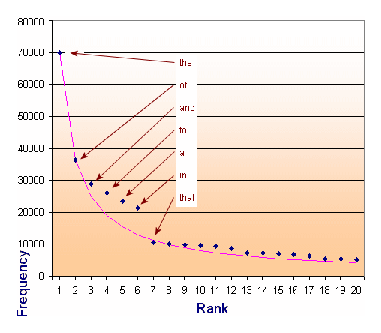
\includegraphics[height=0.9\textheight]{include/bc-0}
\end{center}
\myslide{Is there a general law?}
\begin{itemize}
\item Language after language, corpus after corpus, linguistic
type after linguistic type, . . . we observe the same “few
giants, many dwarves” pattern
\item The nature of this relation becomes clearer if we plot $\log(f)$ as a
function of $\log(r)$
\end{itemize}

\newpage
\begin{center}
  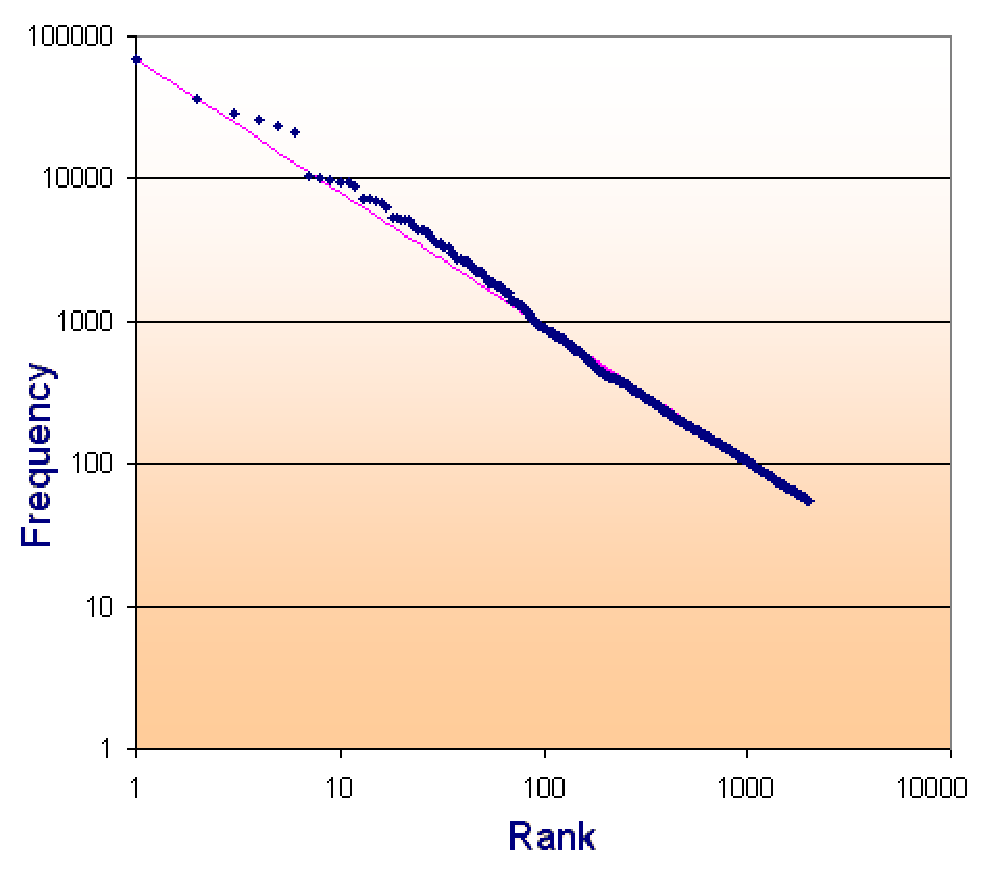
\includegraphics[height=0.98\textheight]{include/bc-2}
\end{center}

\myslide{Zipf's law}

\begin{itemize}
\item Straight line in double-logarithmic space corresponds to
power law for original variables
\item This leads to Zipf's (1949, 1965) famous law:

  \begin{equation}
    \label{eq:1}
    f(w) = \frac{C}{r(w)^a}\ \ \  \textnormal{or} \ \ \  f(w) \propto \frac{1}{r(w)}
  \end{equation}
\\ $f(w)$: Frequency of Word $w$
 \\ $r(w)$: Rank of the Frequency of Word $w$ (most frequent = 1, \ldots)

\begin{itemize}
  \item With a = 1 and C =60,000, Zipf's law predicts that:
\begin{itemize}
  \item most frequent word occurs 60,000 times
  \item second most frequent word occurs 30,000 times
  \item third most frequent word occurs 20,000 times
  \item and there is a long tail of 80,000 words with frequencies
  \item between 1.5 and 0.5 occurrences(!)
  \end{itemize}
\end{itemize}
\end{itemize}

\myslide{Applications of word frequency distributions}
\begin{itemize}
  \item Most important application: extrapolation of vocabulary
size and frequency spectrum to larger sample sizes
\begin{itemize}
  \item productivity (in morphology, syntax, \ldots)
  \item lexical richness
\\ (in stylometry, language acquisition, clinical linguistics, \ldots)
\item practical NLP (est. proportion of OOV words, typos, \ldots)
\end{itemize}
\item Direct applications of Zipf's law in NLP
\begin{itemize}
\item Population model for Good-Turing smoothing \\ If you have not
  seen a word before its probability should probably not be $0$ but
  closer to $\frac{1}{N}$
  \item Realistic prior for Bayesian language modelling
  \end{itemize}
\end{itemize}


\myslide{Other Zipfian (power-law) Distributions}

\begin{itemize}
\item Calls to computer operating systems (length of call)
\item Colors in images
    \\ the basis of most approaches to image compression
  \item City populations 
\\ a small number of large cities, a larger number of smaller cities
\item Wealth distribution 
\\ a small number of people have large amounts of money, large numbers of people have small amounts of money
\item  Company size distribution
\item Size of trees in a forest (roughly)
\end{itemize}
  

% Statistical Analysis of Corpus Data with R
\section{Hypothesis Testing \\ for Corpus Frequency Data}
%  – The Library Metaphor
% Marco Baroni1\& Stefan Evert2
% http://purl.org/stefan.evert/SIGIL
% 1Center

% for Mind/Brain Sciences, University of Trento
% 2Institute of Cognitive Science, University of Osnabrück
\myslide{Some questions}
\begin{itemize}
\item How many passives are there in English?
  \\ What proportion of verbs are in passive voice?
\begin{itemize}
\item a simple, innocuous question at first sight, and not
particularly interesting from a linguistic perspective
\end{itemize}
\item but it will keep us busy for many hours …
\item slightly more interesting version:
  \begin{itemize}
  \item Are there more passives in written English
than in spoken English?
\end{itemize}
\end{itemize}

\myslide{More interesting questions}
\begin{itemize}
\item How often is \eng{kick the bucket} really used idiomatically?
  How often literally?  How often would you expect to be exposed to
  it?
\item What are the characteristics of \txx{translationese}?
\item Do Americans use more split infinitives than
Britons? What about British teenagers?

\item What are the typical collocates of \eng{cat}?
\item Can the next word in a sentence be predicted?
\item Do native speakers prefer constructions that are
grammatical according to some linguistic theory?
\end{itemize}
% ➡ answers are based on the same frequency estimates
% 3

\myslide{Back to our simple question}
\begin{itemize}
\item How many passives are there in English?
\begin{itemize}
\item American English style guide claims that
\begin{itemize}
\item “In an average English text, no more than 15\% of the
sentences are in passive voice. So use the passive
sparingly, prefer sentences in active voice.”

\item \url{http://www.ego4u.com/en/business-english/grammar/passive}
states that only 10\% of English sentences are
passives (as of June 2006)!
\end{itemize}
\item We have doubts and want to verify this claim
\end{itemize}
\end{itemize}

\myslide{Problem \#1}
\begin{itemize}
\item Problem \#1: What is English?
\item Sensible definition: group of speakers
  \begin{itemize}
  \item e.g. American English as language spoken by
    native speakers raised and living in the U.S.
  \item may be restricted to certain communicative situation
  \end{itemize}
\item Also applies to definition of sublanguage
\begin{itemize}
\item dialect (Bostonian, Cockney), social group (teenagers), genre
  (advertising), domain (statistics), \ldots
\end{itemize}
\end{itemize}

\myslide{Intensional vs. extensional}
\begin{itemize}
\item We have given an intensional definition for
the language of interest
\begin{itemize}
\item characterised by speakers and circumstances
\end{itemize}
\item But does this allow quantitative statements?
\begin{itemize}
\item we need something we can count
\end{itemize}
\item Need extensional definition of language
\begin{itemize}
\item i.e. language = body of utterances
  \begin{quote}
“All utterances made by speakers of the
language under appropriate conditions,
plus all utterances they could have made”
\end{quote}
\end{itemize}
\end{itemize}
\myslide{Problem \#2}
\begin{itemize}
\item Problem \#2: What is “frequency”?
\item Obviously, extensional definition of language
must comprise an infinite body of utterances
\begin{itemize}
\item So, how many passives are there in English?
\item ∞ \ldots infinitely many, of course!
\end{itemize}
\item Only relative frequencies can be meaningful
\end{itemize}

\myslide{Relative frequency}
\begin{itemize}
\item How many passives are there …
\begin{itemize}
\item \ldots per million words?
\item \ldots per thousand sentences?
\item \ldots per hour of recorded speech?
\item \ldots per book?
\end{itemize}
\item Are these measurements meaningful?
\end{itemize}

\myslide{Relative frequency}
\begin{itemize}
\item How many passives could there be at the most?
\begin{itemize}
\item every VP can be in active or passive voice
\item frequency of passives is only interpretable by
comparison with frequency of potential passives
\end{itemize}
\item comparison with frequency of potential passives
\begin{itemize}
\item What proportion of VPs are in passive voice?
\item easier: proportion of sentences that contain a passive
\end{itemize}
\item Relative frequency = proportion \txx{$\mathbf{\pi}$}
\end{itemize}


\myslide{Problem \#3}
\begin{itemize}
\item Problem \#3: How can we possibly count
passives in an infinite amount of text?
\item Statistics deals with similar problems:
\begin{itemize}
\item goal: determine properties of large population
\\(human populace, objects produced in factory, \ldots
\item method: take (completely) random sample of
objects, then extrapolate from sample to population
\item this works only because of random sampling!
\end{itemize}
\item Many statistical methods are readily available
\end{itemize}


\myslide{Statistics \& language}
\begin{itemize}
\item Apply statistical procedure to linguistic problem
  \begin{itemize}
  \item take random sample from (extensional) language
  \item What are the objects in our population?
    \begin{itemize}
    \item words? sentences? texts? …
    \end{itemize}
  \item Objects = whatever proportions are based on
    \into unit of measurement
  \end{itemize}
\item We want to take a random sample of these units
\end{itemize}

\myslide{Types vs. tokens}
\begin{itemize}
\item Important distinction between types \& tokens
\begin{itemize}
\item we might find many copies of the “same” VP in our
sample, e.g. \eng{click this button (software manual)} or
\eng{includes dinner, bed and breakfast}
\end{itemize}
\item sample consists of occurrences of VPs, called tokens
\\ - each token in the language is selected at most once
\item distinct VPs are referred to as types
\\ - a sample might contain many instances of the same type
\item Definition of types depends  on the research question
\end{itemize}

\myslide{Types vs. tokens}
\begin{itemize}
\item Example: \textbf{Word Frequencies}
\begin{itemize}
\item word type = dictionary entry (distinct word)
\item word token = instance of a word in library texts
\end{itemize}
\item Example: \textbf{Passives}
\begin{itemize}
\item relevant VP types = active or passive (\into abstraction)
\item VP token = instance of VP in library texts
\end{itemize}
\end{itemize}

\myslide{Types, tokens and proportions}
\begin{itemize}
\item Proportions in terms of types \& tokens
\item Relative frequency of type $v$
\\ = proportion of tokens $t_i$ that belong to this type

\begin{equation}
  \label{eq:2}
   p = \frac{f(v)}{n}
\end{equation}
\begin{itemize}
\item $f(v) = $ frequency of type
\item $n = $ sample size
\end{itemize}
\end{itemize}



\myslide{Inference from a sample}
\begin{itemize}
\item Principle of inferential statistics
\begin{itemize}
\item if a sample is picked at random, proportions should be
roughly the same in the sample and in the population
\end{itemize}
\item Take a sample of, say, 100 VPs
\begin{itemize}
\item observe 19 passives \into $p = 19\% = .19$
\item style guide \into population proportion $\pi = 15\%$
\item $p > \pi$ \into reject claim of style guide?
\end{itemize}
\item Take another sample, just to be sure
\begin{itemize}
\item observe 13 passives \into $p = 13\% = .13$
\item $p < \pi$ \into claim of style guide confirmed?
\end{itemize}
\end{itemize}

\myslide{Problem \#4}
\begin{itemize}
\item Problem \#4: Sampling variation
  \begin{itemize}
  \item random choice of sample ensures proportions are the
    same on average in sample and in population
\item but it also means that for every sample we will get a
different value because of chance effects
\into \txx{sampling variation}
\end{itemize}
\item The main purpose of statistical methods is to
estimate \& correct for sampling variation
\begin{itemize}
\item that's all there is to statistics, really \smiley
\end{itemize}
\end{itemize}

\myslide{Estimating sampling variation}
\begin{itemize}
\item Assume that the style guide's claim is correct
\begin{itemize}
\item the null hypothesis $H_0$, which we aim to refute
\\ \[H_0:\pi = .15 \]
\item we also refer to $\pi_0$ = .15 as the null proportion
\end{itemize}
\item Many corpus linguists set out to test $H_0$
\begin{itemize}
\item each one draws a random sample of size $n = 100$
\item how many of the samples have the expected $k = 15$
passives, how many have $k = 19$, etc.?
\end{itemize}
\end{itemize}

\myslide{Estimating sampling variation}
\begin{itemize}
\item We don't need an infinite number of monkeys
(or corpus linguists) to answer these questions
\begin{itemize}
\item randomly picking VPs from our metaphorical library
is like drawing balls from an infinite urn
\item red ball = passive VP / white ball = active VP
\item $H_0$: assume proportion of red balls in urn is 15%
\end{itemize}
\item This leads to a binomial distribution
\[ \frac{(\pi_0)(1 - \pi_0)}{N} \]
\end{itemize}



\myslide{Binomial Sampling Distribution for $N=20, \pi=.4$}

\begin{center}
  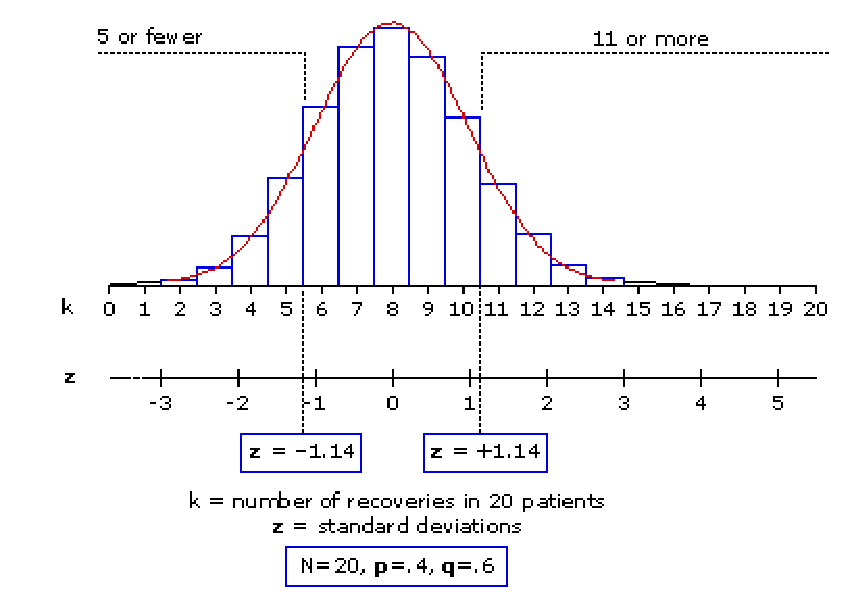
\includegraphics[height=0.98\textheight]{include/binom.eps}
\end{center}


\myslide{Statistical hypothesis testing}
\begin{itemize}
\item Statistical hypothesis tests
\begin{itemize}
\item define a rejection criterion for refuting $H_0$
\item control the risk of false rejection (type I error) to a
“socially acceptable level” (significance level)
\item p-value = risk of false rejection for observation
\item p-value interpreted as amount of evidence against $H_0$
\end{itemize}
\item Two-sided vs. one-sided tests
\begin{itemize}
\item in general, two-sided tests should be preferred
\item one-sided test is plausible in our example
\end{itemize}
\end{itemize}


% \myslide{Evaluation Metrics}
% %%%

% \begin{description}
% \item[Precision] Ratio of correctly labeled/Labeled (\blu{P}: Accuracy)
% \item[Recall] Ratio of correctly labeled/Should have been labeled (\blu{R})
% \end{description}

% Normally we can raise precision at the cost of lower recall and vice-versa.  So we try to optimize a combined score: \txx{F-measure}

% \begin{description}
% \item[F-measure] A  measure of overall goodness
% $\frac{2PR}{P+R}$ (\blu{F})
% \end{description}

% More generally F-measure is $\frac{(1+\beta^2)PR}{\beta^2P+R}$.  

% Most often we set $\beta=1$.  If Precision is more important, increase $\beta$.



\myslide{Error Types}


\begin{tabular}{l|cc}
  System        & \multicolumn{2}{c}{Actual} \\
          & target & not target \\ \hline
  selected      & tp     & \emp{fp} \\  
  not selected  & \emp{fn}     & tn 
\end{tabular}

Precision $=\frac{tp}{tp+fp}$; Recall $=\frac{tp}{tp+fn}$; F$_1$ $=\frac{2PR}{P+R}$


\begin{description} \addtolength{\itemsep}{-1ex}
\item[tp] True positives: system says Yes, target was Yes
\item[fp] False positives: system says Yes, target was No  (Type I Error)
\item[tn] True negatives: system says No, target was No
\item[fn] False negatives: system says No, target was Yes  (Type II Error)
\end{description}

\myslide{Example: Similarity}

\begin{itemize}
\item System says \eng{eggplant} is similar to \eng{brinjal}
  \\ \blu{True positive} 
\item System says \eng{eggplant} is similar to \eng{egg}
  \\ depends on the application (both food), but generally not so good
  \\ \emp{False positive}
\item System says \eng{eggplant} is \textbf{not} similar to \eng{aubergine}
  \\ \emp{False negative}
\item System says \eng{eggplant} is \textbf{not} similar to \eng{laptop}
  \\ \blu{True negative}
\end{itemize}





\myslide{Hypothesis tests in practice}
\begin{itemize}
\item Easy: use online wizard 
  \begin{itemize}
  \item \url{http://sigil.collocations.de/wizard.html}
  \item \url{http://vassarstats.net/}
\end{itemize}
\item Or \txx{Python}
  \begin{itemize}
  \item One-tail test: \texttt{scipy.stats.binom.sf(k, n, p)}
    \\ k = number of successes, p = number of trials, 
    \\ p = hypothesized     probability of success
    \\ returns p-value of the hypothesis test
  \item Two-tail test:  \texttt{scipy.stats.binom\_test(k,n,p)}
  \end{itemize}
\item Or \txx{R} \url{http://www.r-project.org/}

\end{itemize}


\myslide{Confidence interval}
 \begin{itemize}
 \item We now know how to test a null hypothesis $H_0$,
   rejecting it only if there is sufficient evidence
 \item But what if we do not have an obvious
   null hypothesis to start with?
   \begin{itemize}
 \item this is typically the case in (computational) linguistics
 \end{itemize}
\item We can estimate the true population proportion
from the sample data (relative frequency)
\begin{itemize}
\item sampling variation \into range of plausible values
\item such a confidence interval can be constructed by
inverting hypothesis tests (e.g. binomial test)
\end{itemize}
\end{itemize}

\myslide{Confidence intervals}
\begin{itemize}
\item Confidence interval = range of plausible values
for true population proportion
\\ We know the answer is almost certainly more than X and less than Y
\item Size of confidence interval depends on sample
size and the significance level of the test
\item The larger your sample, the narrower the interval will be
\\ that is the more accurate your estimate is
\begin{itemize}
\item $19/100$ \into 95\% confidence interval: 	[12.11\% … 28.33\%] 
\item $190/1000$ \into 95\% confidence interval: [16.64\% … 21.60\%] 
\item $1900/10000$ \into 95\% confidence interval: [18.24\% … 19.79\%] 
\end{itemize}
\item \url{http://sigil.collocations.de/wizard.html}
\end{itemize}
\myslide{Effect Size}
\MyLogo{\href{https://xkcd.com/882/}{Green Jelly Beans linked to Acne!}}
\begin{itemize}
\item The difference between the two values is the effect size
\item For something to be significant the two confidence intervals
  should not overlap
  \begin{itemize}
  \item either a small confidence interval (more data)
  \item or a big effect size (clear difference)
  \end{itemize}
\item lack of significance does not mean that there is no difference
  only that we are not sure
\item significance does not meant that there is a difference only that
  it is unlikely to be by chance
\item if we run an experiment with 20 different configurations and one
  is significant what does this tell us?

\end{itemize}

\myslide{Frequency comparison}
\begin{itemize}
\item Many linguistic research questions can be
operationalised as a frequency comparison
\begin{itemize}
\item Are split infinitives more frequent in AmE than BrE?
\item Are there more definite articles in texts written by
Chinese learners of English than native speakers?
\item Does \eng{meow} occur more often in the vicinity of \eng{cat}
than elsewhere in the text?
\item Do speakers prefer \eng{I couldn't agree more} over
alternative compositional realisations?
\end{itemize}
\item Compare observed frequencies in two samples
\end{itemize}


\myslide{Frequency comparison}

\begin{tabular}{|c|c|}
\hline
  $k_1 $ & $k_2 $ \\
\hline
  $n_1 - k_1 $ & $n_2 - k_2 $ \\
\hline
\end{tabular}
\begin{tabular}{|c|c|}
\hline
  19 & 25 \\
\hline
  81 & 175 \\ 
\hline
\end{tabular}

\begin{itemize}
\item Contingency table for frequency comparison
\begin{itemize}
\item e.g. samples of sizes $n_1$ = 100 and $n_2$ = 200,
containing 19 and 25 passives
\item $H_0$: same proportion in both underlying populations
\end{itemize}
\item Chi-squared $X^2$, likelihood ratio $G^2$, Fisher's test
  \begin{itemize}
  \item based on same principles as binomial test
  \end{itemize}
\end{itemize}


\myslide{Frequency comparison}
\begin{itemize}
\item Chi-squared, log-likelihood and Fisher are
appropriate for different (numerical) situations

\item Estimates of effect size (confidence intervals)
\begin{itemize}
\item e.g. difference or ratio of true proportions
\item exact confidence intervals are difficult to obtain
\item log-likelihood seems to do best for many corpus measures
\end{itemize}
\item Frequency comparison in practice
\begin{itemize}
\item \url{http://sigil.collocations.de/wizard.html}
\end{itemize}
\end{itemize}

\myslide{Do Particle verbs correlate with compound verbs?}
\MyLogo{For more details see Soh, Xue Ying Sandra (2015)}
\begin{itemize}
\item Compound verbs: 光り輝く \jpn[shine-sparkle]{hikari-kagayaku}; 
  書き上げる \jpn[write up (lit: write-rise)]{kaki-ageru}
\item Particle Verbs: \eng{give up}, \eng{write up}
\item Look at all verb pairs from Wordnet \\
  \begin{tabular}{l|rr}
      & PV & V \\ \hline
   VV &  1,777 & 5,885 \\     
   V  &  10,877 & 51,137 
  \end{tabular}
\item Questions:
  \begin{itemize}
  \item What is the confidence interval for the distribution of VV in Japanese?
  \item What is the confidence interval for the distribution of PV in English?
  \item How many PV=VV would you expect if they were independent?
  \item Is PV translated as VV more than chance?
  \end{itemize}
\end{itemize}


\section{Collocations}
%\lurl{???}
% Statistical Analysis of Corpus Data with R
% You shall know a word by the company it keeps!
% Collocation extraction with statistical association measures
% — Part 1 —
% Designed by Marco Baroni1 and Stefan Evert2
% 1 Center

% for Mind/Brain Sciences (CIMeC)
% University of Trento

% 2 Institute

% of Cognitive Science (IKW)
% University of Onsabrück

\myslide{Outline}
\begin{itemize}
\item Collocations \& Multiword Expressions (MWE)
\begin{itemize}
\item What are collocations?
\item Types of cooccurrence
\end{itemize}
\item Quantifying the attraction between words
\begin{itemize}
\item Contingency tables
\end{itemize}
\end{itemize}

% \item Contingency tables and hypothesis tests in R
%Practice session

\myslide{What is a collocation?}
\MyLogo{My grand-supervisor: Bond - Huddleston - Halliday - Firth}
\begin{itemize}
\item Words tend to appear in typical, recurrent combinations:
\begin{itemize}
\item \eng{day} and \eng{night}
\item \eng{ring} and \eng{bell}
\item \eng{milk} and \eng{cow}
\item \eng{kick} and \eng{bucket}
\item \eng{brush} and \eng{teeth}
\end{itemize}
\item such pairs are called \txx{collocations} \citep{Firth:1957}
\item the meaning of a word is in part determined by its
characteristic collocations
\begin{quote}
``You shall know a word by the company it keeps!''
\end{quote}
\end{itemize}

\myslide{What is a collocation?}

\begin{itemize}
\item Native speakers have strong and widely shared intuitions
about such collocations
\begin{itemize}
\item Collocational knowledge is essential for non-native
speakers in order to sound natural
\item This is part of ``idiomatic language''
\end{itemize}
\end{itemize}

\myslide{An important distinction}

\begin{itemize}
\item \txx{Collocations} are an empirical linguistic phenomenon
\begin{itemize}
\item can be observed in corpora and quantified
\item provide a window to lexical meaning and word usage
\item applications in language description (Firth 1957) and
computational lexicography \citep{Sinclair:1991}
\end{itemize}
\item \txx{Multiword expressions} = lexicalised word combinations
\begin{itemize}
\item MWE need to be lexicalised (i.e., stored as units) because
of certain idiosyncratic properties
\item non-compositionallity, non-substitutability, non-modifiability
  \citep{Manning:Schuetze:1999}
\item not directly observable, defined by linguistic tests
(e.g. substitution test) and native speaker intuitions
\item Sometimes called \txx{collocations} but we will distinguish
\end{itemize}
\end{itemize}

\myslide{But what are collocations?}
\MyLogo{\eng{epiphenomenon} ``a secondary phenomenon that is a by-product of
  another phenomenon''}

\begin{itemize}
\item   Empirically, collocations are words that show an attraction towards
  each other (or a \txx{mutual expectancy}) 
\begin{itemize}
\item in other words, a tendency to
  occur near each other
\item  collocations can also be understood as
  statistically salient patterns that can be exploited by language
  learners
\end{itemize}
\item Linguistically, collocations are an epiphenomenon of many
  different linguistic causes that lie behind the observed surface
  attraction.   

\end{itemize}

\myslide{Collocates of \lex{bucket} (n.)}
\begin{small}
  \vspace*{0.5ex}\begin{tabular}{lrlrlr}
    noun       & f    & verb       & f   & adjective     & f   \\   \hline
    water      & 183  & throw      & 36  & large         & 37  \\ 
    spade      & 31   & fill        & 29  & single-record & 5   \\ 
    plastic    & 36   & randomize  & 9   & cold          & 13  \\ 
    slop       & 14   & empty      & 14  & galvanized    & 4   \\ 
    size       & 41   & tip        & 10  & ten-record    & 3   \\ 
    mop        & 16   & kick       & 12  & full          & 20  \\ 
    record     & 38   & hold       & 31  & empty         & 9   \\ 
    bucket     & 18   & carry      & 26  & steaming      & 4   \\ 
    ice        & 22   & put        & 36  & full-track    & 2   \\ 
    seat       & 20   & chuck      & 7   & multi-record  & 2   \\ 
    coal       & 16   & weep       & 7   & small         & 21  \\ 
    density    & 11   & pour       & 9   & leaky         & 3   \\ 
    brigade    & 10   & douse      & 4   & bottomless    & 3   \\ 
    algorithm  & 9    & fetch      & 7   & galvanised    & 3   \\ 
    shovel     & 7    & store      & 7   & iced          & 3   \\ 
    container  & 10   & drop       & 9   & clean         & 7   \\ 
    oats       & 7    & pick       & 11  & wooden        & 6   \\ 
%    sand       & 12   & use        & 31  & old           & 19  \\ 
%    Rhino      & 7    & tire       & 3   & ice-cold      & 2   \\ 
%    champagne  & 10   & rinse      & 3   & anti-sweat    & 1   \\ 
  \end{tabular}
\end{small}\vspace*{-1.0ex}


 
\myslide{Collocates of bucket (n.)}
\begin{itemize}
\item opaque \txx{idioms} 
  (\eng{kick the bucket}, but often used literally)
\item \txx{proper names} 
  (\eng{Rhino Bucket}, a hard rock band)
\item \txx{noun compounds}, lexicalised or productively formed
\\(\eng{bucket shop, bucket seat, slop bucket, champagne bucket})
\item \txx{lexical collocations} = semi-compositional combinations
\\(\eng{weep buckets, brush one's teeth, give a speech})
\item cultural \txx{stereotypes} 
  (\eng{bucket and spade})
\item \txx{semantic compatibility} (\eng{full, empty, leaky \ul{bucket};
throw, carry, fill, empty, kick, tip, take, fetch a \ul{bucket}})
\item \txx{semantic fields} (\eng{shovel, mop}; hypernym \eng{container})
\item \txx{facts of life} (\eng{wooden bucket; bucket of water, sand, ice, \ldots} )
\item often sense-specific (\eng{bucket size, randomize to a bucket})
\end{itemize}

\myslide{Operationalising collocations}
\begin{itemize}
\item Firth introduced collocations as an essential component of
his methodology, but without any clear definition
\begin{quote}
  Moreover, these and other technical words are given their ‘meaning'
  by the restricted language of the theory, and by applications of the
  theory in quoted works. (Firth 1957, 169)
\end{quote}
\item Empirical concept needs to be formalised and quantified
  \begin{itemize}%\addtolength{\itemsep}{-0.5ex}
  \item intuition: collocates are “attracted” to each other, 
    \\ i.e. they tend to occur near each other in text
  \item definition of “nearness” \into cooccurrence
  \item quantify the strength of attraction between collocates based
    on their recurrence \into cooccurrence frequency
\item We will consider word pairs $(w_1, w_2)$ such as 
(\eng{brush, teeth})

\end{itemize}
  \end{itemize}


\myslide{Different types of cooccurrence}
\begin{enumerate}
\item  \txx{Surface cooccurrence}
  \begin{itemize}
  \item criterion: surface distance measured in word tokens
  \item words in a \txx{collocational span} (or \txx{window}) around
    the node word, may be symmetric (L5, R5) or asymmetric (L2, R0)
  \item  traditional approach in lexicography and corpus linguistics
  \end{itemize}
\item \txx{Textual cooccurrence}
  \begin{itemize}
\item words cooccur if they are in the same text segment
\\ (sentence, paragraph, document, Web page, . . . )
\item often used in Web-based research (\into Web as corpus)
\item often used in indexing
\end{itemize}
\newpage
\item \txx{Syntactic cooccurrence}
  \begin{itemize}
  \item words in a specific syntactic relation
  \begin{itemize}
  \item adjective modifying noun
  \item subject/object noun of verb
  \item \textit{N of N} 
  \end{itemize}
\item suitable for extraction of MWEs (Krenn and Evert 2001)
\end{itemize}
\item[*] Of course you can combine these
\end{enumerate}

\myslide{Surface cooccurrence}

\begin{itemize}
  \item Surface cooccurrences of 
    $w_1$ = \eng{hat} with $w_2$ = \eng{roll}
  \item symmetric window of four words (L4, R4)
  \item  limited by sentence boundaries
  \end{itemize}
  
  \begin{quotation}
A vast deal of coolness and a peculiar degree of judgement, are requisite in catching a \blu{hat} . A man must
not be precipitate, or he runs over it ; he must not rush into the opposite extreme, or he loses it
altogether. [. . . ] There was a fine gentle \ul{wind, and Mr. Pickwick's \blu{hat} \emp{rolled} sportively before it} . The
wind puffed, and Mr. \ul{Pickwick puffed, and the \blu{hat} \emp{rolled} over and over} as merrily as a lively porpoise
in a strong tide ; and on it might have \emp{rolled}, far beyond Mr. Pickwick's reach, had not its course been
providentially stopped, just as that gentleman was on the point of resigning it to its fate.
  \end{quotation}
  \begin{itemize}
  \item coocurrence frequency $f$ = 2
  \item marginal frequencies $f_1$(hat) = $f_2$(roll) = 3
  \end{itemize}
  
\myslide{Textual cooccurrence}
\begin{itemize}
 \item Surface cooccurrences of 
    $w_1$ = \eng{hat} with $w_2$ = \eng{over}
  \item textual units = sentences
  \item multiple occurrences within a sentence ignored
  \end{itemize}
  \begin{small}
    \begin{tabular}{p{0.8\textwidth}ll}
      A vast deal of coolness and a peculiar degree of judgement, are
      requisite in catching a hat.
      &
      hat
      &
      —
      \\
      A man must not be precipitate, or he runs over it ;
      &
      —
      &
      over
      \\
      he must not rush into the opposite extreme, or he loses it
      altogether.
      &
      —
      &
      —
      \\
      There was a fine gentle wind, and Mr. Pickwick's hat rolled
      sportively before it.
      &
      hat
      &
      —
      \\
      The wind puffed, and Mr. Pickwick puffed, and the hat rolled
      over and over as merrily as a lively porpoise in a strong tide ;
      &
      hat
      &
      over
    \end{tabular}
  \end{small}

\begin{itemize}
\item coocurrence frequency $f = 1$
\item marginal frequencies $f_1$ = 3, $f_2$ = 2
\end{itemize}

\myslide{Syntactic cooccurrence}

\begin{itemize}
\item Syntactic cooccurrences of adjectives and nouns
\item every instance of the syntactic relation (A-N) is
extracted as a pair token
\end{itemize}



\begin{itemize}
\item  Cooccurrency frequency data for young gentleman:
  \begin{small}
    \begin{itemize}
    \item \eng{There were two gentlemen who came to see you.}  \\ (\eng{two,
      gentleman})
    \item \eng{He was no gentleman, although he was young.}  \\ (\eng{no,
      gentleman}) (\eng{young, he})
    \item \eng{The old, stout gentleman laughed at me.}  \\ (\eng{old, gentleman})
      (\eng{stout, gentleman})
    \item \eng{I hit the young, well-dressed gentleman.}  
      \\ (\eng{young,    gentleman}) (\eng{well-dressed gentleman})
    \end{itemize}
  \end{small}
 \begin{itemize}
    \item coocurrence frequency $f = 1$
    \item marginal frequencies $f_1 = 2, f_2 = 6$
\end{itemize}
\end{itemize}
\myslide{Quantifying attraction}
\begin{itemize}
\item Quantitative measure for attraction between words based
on their recurrence \into \txx{cooccurrence frequency}
\item 
But cooccurrence frequency is not sufficient
\begin{itemize}
\item bigram \eng{is to} occurs $f = 260$ times in Brown corpus
\item but both components are so frequent ($f_1 \approx   10,000$ and
$f_2 \approx   26,000$) that one would also find the bigram 260 times if
words in the text were arranged in completely random order

\item take expected frequency into account as \txx{baseline}
\end{itemize}
\item 
Statistical model required to bring in notion of \txx{chance
cooccurrence} and to adjust for sampling variation
\\ bigrams can be understood either as syntactic
cooccurrences (adjacency relation) or as surface
cooccurrences (L1, R0 or L0, R1)
\end{itemize}

\myslide{What is an $n$-gram?}
\begin{itemize}
\item An $n$-gram is a subsequence of $n$ items from a given
  sequence. The items in question are typically phonemes, syllables, letters,
  words or base pairs according to the application.
  \begin{itemize}
  \item $n$-gram of size 1 is referred to as a \txx{unigram};
  \item size 2 is a \txx{bigram} (or, less commonly, a \txx{digram})
  \item size 3 is a \txx{trigram}
  \item size 4 or more is simply called an \txx{$n$-gram}
\end{itemize}
\item \txx{bigrams} (from the first sentence):
BOS \eng{An,  An $n$-gram, $n$-gram is, is a, a subsequence, subsequence of, \ldots}
\item \txx{$4$-grams} (from the first sentence):
BOS \eng{An $n$-gram is, An $n$-gram is a, $n$-gram is a subsequence, is a subsequence of, \ldots}
\end{itemize}

\myslide{Attraction as statistical association}
\begin{itemize}
\item Tendency of events to cooccur = \txx{statistical association}
\begin{itemize}
\item statistical measures of association are available for
contingency tables, resulting from a cross-classification
of a set of “items” according to two (binary) factors
cross-classifying factors represent the two events
\end{itemize}
\item Application to word cooccurrence data
\begin{itemize}

\item most natural for syntactic cooccurrences
\item ``items'' are pair tokens $(x, y)$ = instances of syntactic relation
\item factor 1: Is $x$ an instance of word type $w_1$?
\item factor 2: Is $y$ an instance of word type $w_2$?
\end{itemize}
\end{itemize}

\myslide{Measuring association in contingency tables}


\begin{tabular}{lcc}
     & $w_1$ & $\neg w_1$ \\
   $w_2$ & both & one \\ 
$\neg w_2$ & other & neither 
\end{tabular}


\begin{itemize}
\item Measures of significance
\begin{itemize}
\item
apply statistical hypothesis test with null hypothesis $H_0$ :
independence of rows and columns
\item $H_0$ implies there is no association between $w_1$ and $w_2$
\item association score = test statistic or p-value
\item one-sided vs. two-sided tests
\item[\into] amount of evidence for association between $w_1$ and $w_2$
\end{itemize}
\newpage
\item Measures of effect-size
\begin{itemize}
\item compare observed frequencies $O_{ij}$ to expected
frequencies $E_{ij}$ under $H_0$
\item  or estimate conditional prob. Pr($w_2$ | $w_1$ ), Pr($w_1$ | $w_2$ ), etc.
\item maximum-likelihood estimates or confidence intervals
\item[\into] strength of the attraction between $w_1$ and $w_2$
\end{itemize}
\end{itemize}

\myslide{Interpreting hypothesis tests as association scores}
\begin{itemize}
\item Establishing significance
  \begin{itemize}
  \item p-value = probability of observed (or more “extreme”)
contingency table if $H_0$ is true
\item theory: $H_0$ can be rejected if p-value is below accepted
significance level (commonly .05, .01 or .001)
\item practice: nearly all word pairs are highly significant
\end{itemize}
\newpage
\item Test statistic = significance association score
\begin{itemize}
\item convention for association scores: high scores indicate
strong attraction between words
\item Fisher's test: transform p-value, e.g.$-log_{10}$p
\item satisfied by test statistic $X^2$, but not by p-value
\item Also log-likelihood $G^2$
\end{itemize}
\item In practice, you often just end up ranking candidates
  \\ different measures give similar results
  \\ there is no perfect statistical score
\end{itemize}


\myslide{Acknowledgments}

 \begin{itemize}
 \item Thanks to Stefan Th. Gries (University of California, Santa
   Barbara) for his great introduction \textit{Useful statistics for
     corpus linguistics}:
\url{https://pdfs.semanticscholar.org/069f/d4b980d75af1125afa2ac3c8f5af2e66414d.pdf}

 \item Many slides inspired by Marco Baroni and Stefan Evert's
   \textbf{SIGIL} \textit{A gentle introduction to statistics for
   (computational) linguists}
 \\ \url{http://www.stefan-evert.de/SIGIL/} 
 \item Some examples taken from Ted Dunning's \textit{Surprise and
     Coincidence - musings from the long tail}
   \url{http://tdunning.blogspot.com/2008/03/surprise-and-coincidence.html}
%   inspiration for some of the slides (from  \textit{LING 2050 Special Topics in Linguistics: Corpus linguistics}, U Penn).
% \item Thanks to Sandra K\"{u}bler for some of the slides from her 
% \textit{RoCoLi\footnote{Romania Computational Linguistics Summer School} Course: Computational Tools for Corpus Linguistics}
% %\item Thanks to Mark Davies (BYU) for the exploration ideas.
% \item Definitions from WordNet 3.0
 \end{itemize}

\end{document}

%%% Local Variables: 
%%% coding: utf-8
%%% mode: latex
%%% TeX-PDF-mode: t
%%% TeX-engine: xetex
%%% LaTeX-section-list:  (("myslide" 1))
%%% End: 